% This is text associated with the open textbook "Open Electromagnetics"
% See immediately below for author, date
% This work is licensed under the Creative Commons Attribution-ShareAlike 4.0 International License. (CC BY SA 4.0) 
% To view a copy of the license, visit http://creativecommons.org/licenses/by-sa/4.0/

%ORB TITLE Transformers as Two-Port Devices
%ORB AUTHOR 0        # S.W. Ellingson, Virginia Tech (ellingson@vt.edu)
%ORB DATE 20180807   # yyyymmdd
%ORB ABSTRACT Transformers as Two-Port Devices

\label{m0032_Transformers_as_Two-Port_Devices} % <-- Must match name of this file and module directory name.  Don't mess with this!
\index{transformer|(}

Section~\ref{m0031_Transformers_Principle_of_Operation} explains the principle of operation of the ideal transformer.
The relationship governing the terminal voltages $V_1$ and $V_2$ was found to be
%
\begin{equation}   
\frac{V_1}{V_2} = p\frac{N_1}{N_2}
\end{equation}
%
where $N_1$ and $N_2$ are the number of turns in the associated coils and $p$ is either $+1$ or $-1$ depending on the relative orientation of the windings; i.e., whether the reference direction of the associated fluxes is the same or opposite, respectively. 
 
We shall now consider ratios of current and impedance in ideal transformers, using the two-port model shown in Figure~\ref{m0032_f2P}.  
By virtue of the reference current directions and polarities chosen in this figure, the power delivered by the source $V_1$ is $V_1 I_1$, and the power absorbed by the load $Z_2$ is $-V_2 I_2$.  Assuming the transformer windings have no resistance, and assuming the magnetic flux is perfectly contained within the core, the power absorbed by the load must equal the power provided by the source; i.e., $V_1 I_1 = -V_2 I_2$.  Thus, we have\footnote{
The minus signs in this equation are a result of the reference polarity and directions indicated in Figure~\ref{m0032_f2P}.
These are more-or-less standard in electrical two-port theory (see ``Additional Reading'' at the end of this section), but are certainly not the only reasonable choice.
If you see these expressions without the minus signs, it probably means that a different combination of reference directions/polarities is in effect.
} % \footnote
%
\begin{equation}   
\boxed{
\frac{I_1}{I_2} = -\frac{V_2}{V_1} = -p\frac{N_2}{N_1}
}
\end{equation}
%
\begin{figure}[b!]
\begin{center}
\pdftooltip{{  % note double braces
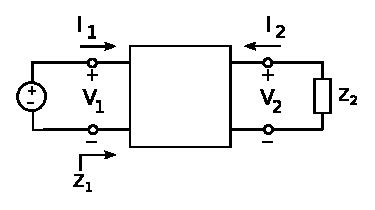
\includegraphics[width=2.5in]{modules/m0032_f2P.eps}
}}{A transformer between two circuits, one on the left and one on the right. In the left circuit is an independent voltage source between a positive and negative node. Between the nodes is labeled V sub 1. From the positive node, I sub 1 is shown going into the transformer. From the negative node Z sub 1 is shown going into the transformer. In the right circuit is an impedance, Z sub 2, between a positive and negative node labeled V sub 2.  From the positive node, I sub 2 is shown going into the transformer.}
\end{center} 
\caption{\label{m0032_f2P} The transformer as a two-port circuit device.}
\end{figure} 

We can develop an impedance relationship for ideal transformers as follows. 
Let $Z_1$ be the input impedance of the transformer; that is, the impedance looking into port~1 from the source.
Thus, we have
%
\begin{flalign}
Z_1 &\triangleq \frac{V_1}{I_1} \nonumber \\ 
    &= \frac{+p\left(N_1/N_2\right)V_2}{-p\left(N_2/N_1\right)I_2} \nonumber \\
    &= -\left(\frac{N_1}{N_2}\right)^2\left(\frac{V_2}{I_2}\right)
\end{flalign}
%
In Figure~\ref{m0032_f2P}, $Z_2$ is the the output impedance of port 2; that is, the impedance looking out port 2 into the load.
Therefore, $Z_2 = -V_2/I_2$ (once again the minus sign is a result of our choice of sign conventions in Figure~\ref{m0032_f2P}).
Substitution of this result into the above equation yields
%
\begin{equation}
Z_1 = \left(\frac{N_1}{N_2}\right)^2 Z_2
\end{equation}
%
and therefore
%
\begin{equation}
\boxed{
\frac{Z_1}{Z_2} = \left(\frac{N_1}{N_2}\right)^2 
}
\end{equation}
%
Thus, we have demonstrated that a transformer scales impedance in proportion to the square of the turns ratio $N_1/N_2$.
Remarkably, the impedance transformation depends \emph{only} on the turns ratio, and is independent of the relative direction of the windings ($p$). 

%The voltage ratio, current ratio, and impedance ratio laws for ideal transformers are often sufficient for analysis and design of circuits using practical transformers.  Sometimes however the non-ideal aspects of transformers must be also be considered.  
%There are two mechanisms which may impact the performance of a transformer:  {\it Winding capacitance} and {\it stray inductance}.  These additional mechanisms are indicated in the equivalent circuit shown in Figure~\ref{fTF-DCM} as $C_{ic}$ and $L_{stray}$ respectively.  Winding capacitance is due to the storage of electric energy in the space between the individual turns of the coil.   
%Stray inductance results from the imperfect containment of the magnetic flux.  
%In particular, magnetic flux generated near the ends of the coils may exist in small loops that do not pass through the other coil, in which case that portion of the coil is behaving as a simple inductor as opposed to a transformer.  
%%
%\begin{figure}
%%\begin{center}\psfig{file=figs/101025_LWA1_HighRes_trim.eps,width=6.3in}\end{center} 
%\vspace{3in}
%\caption{\label{m0032_f2PEC} Circuit model for a transformer including winding capacitance and stray inductance.}
%\end{figure} 

The relationships developed above should be viewed as AC expressions, and are not normally valid at DC.
This is because transformers exhibit a fundamental limitation in their low-frequency performance.
To see this, first recall Faraday's Law:
%
\begin{equation}   
V = - N \frac{\partial}{\partial t} \Phi
\end{equation}
%
If the magnetic flux $\Phi$ isn't time-varying, then there is no induced electric potential, and subsequently no linking of the signals associated with the coils.
At very low but non-zero frequencies, we encounter another problem that gets in the way -- \emph{magnetic saturation}.
\index{saturation (magnetic)}
To see this, note we can obtain an expression for $\Phi$ from Faraday's Law by integrating with respect to time, yielding
%
\begin{equation}
\Phi(t) = -\frac{1}{N}\int_{t_0}^{t}V(\tau)d\tau + \Phi(t_0)   
\end{equation}
%
where 
$t_0$ is some earlier time at which we know the value of $\Phi(t_0)$.
Let us assume that $V(t)$ is sinusoidally-varying.
Then the peak value of $\Phi$ after $t=t_0$ depends on the frequency of $V(t)$.  
If the frequency of $V(t)$ is very low, then $\Phi$ can become very large.  Since the associated cross-sectional areas of the coils are presumably constant, this means that the magnetic field becomes very large.  The problem with that is that most practical high-permeability materials suitable for use as transformer cores exhibit magnetic saturation; that is, the rate at which the magnetic field is able to increase decreases with increasing magnetic field magnitude (see Section~\ref{m0058_Magnetic_Materials}).  
The result of all this is that a transformer may work fine at (say) 1~MHz, but at (say) 1~Hz the transformer may exhibit an apparent loss associated with this saturation.  Thus, practical transformers exhibit highpass frequency response. 

It should be noted that the highpass behavior of practical transistors can be useful. For example, a transformer can be used to isolate an undesired DC offset and/or low-frequency noise in the circuit attached to one coil from the circuit attached to the other coil.  

The DC-isolating behavior of a transformer also allows the transformer to be used as a \emph{balun}, 
\index{balun}
as illustrated in Figure~\ref{m0032_fBalun}.  A balun is a two-port device that transforms a single-ended (``unbalanced'') signal -- that is, one having an explicit connection to a datum (e.g., ground) -- into a differential (``balanced'') signal, for which there is no explicit connection to a datum.  Differential signals have many benefits in circuit design, whereas inputs and outputs to devices must often be in single-ended form.
Thus, a common use of transformers is to effect the conversion between single-ended and differential circuits.
Although a transformer is certainly not the only device that can be used as a balun, it has one very big advantage, namely bandwidth.
%
\begin{figure}
\begin{center}
\pdftooltip{{  % note double braces
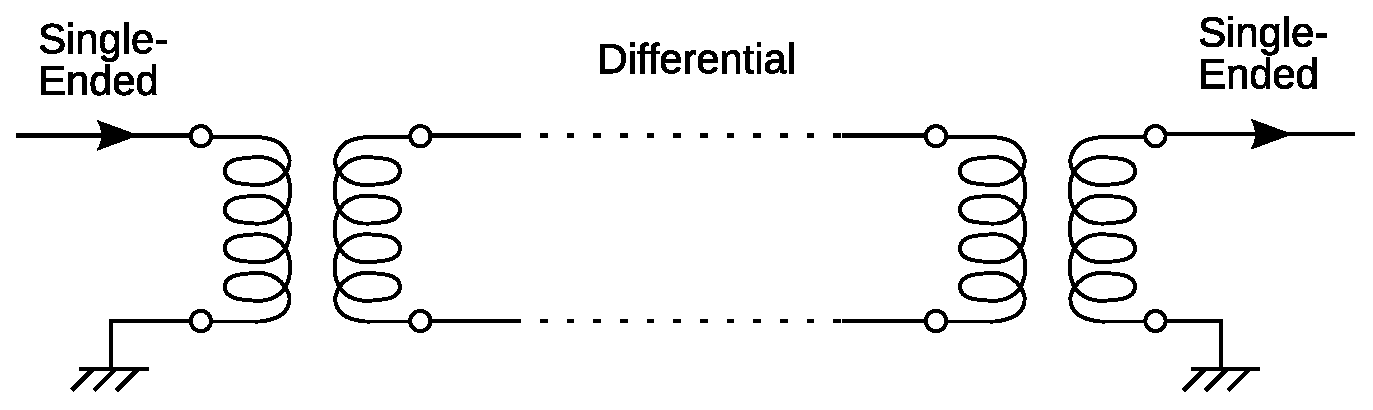
\includegraphics[width=\columnwidth]{modules/m0032_fBalun.eps}
% https://en.wikipedia.org/wiki/File:Transformer_balance.svg
}}{A single-ended coil has current entering the top and the bottom is connected to ground. To its right is a second coil connected to a third coil by a dashed line and labeled differential. To the right of the “differential” is a final single-ended coil with current exiting to the top and grounded at the bottom.}
\end{center} 
\centerline{\scriptsize 
\copyright~\hyperref[m0032_fBalun_Credit]{SpinningSpark} 
\href{https://creativecommons.org/licenses/by-sa/3.0/}{CC BY~SA 3.0} 
(modified)
} 
\caption{
\label{m0032_fBalun}
Transformers used to convert a single-ended (``unbalanced'') signal to a differential (balanced) signal, and back.
}
\end{figure}

%%%%%%%%%%%%%%%%%%%%%%%%%%%%%%%%%%%%%%%%%%%%%%%%%%%%%%%%%%%%%%%%%%%%%%

{\bf Additional Reading:}
\begin{itemize}
\item ``\href{https://en.wikipedia.org/wiki/Transformer}{Transformer}'' on Wikipedia.
\item ``\href{https://en.wikipedia.org/wiki/Two-port_network}{Two-port network}'' on Wikipedia.
\item ``\href{https://en.wikipedia.org/wiki/Saturation_(magnetic)}{Saturation (magnetic)}'' on Wikipedia.
\item ``\href{https://en.wikipedia.org/wiki/Balun}{Balun}'' on Wikipedia.
\item S.W. Ellingson, ``Differential Circuits'' (Sec.~8.7) in \emph{Radio Systems Engineering}, Cambridge Univ.\ Press, 2016.
\end{itemize}

\index{transformer|)}
